\section{Expressivité du système d'observation}\label{sec:valid:domvision:requetes}
Dans cette section, nous détaillons les capacités d'interrogations d'Astral appliquées sur notre architecture. Tout d'abord, nous détaillons comment le catalogue est entretenu avec les données provenant des flux. Ensuite, nous archivons des données volatiles. Enfin, nous exploitons cet ensemble pour former des requêtes continues de haut niveau.

\subsection{Entretien du catalogue}
Nous avons à notre disposition plusieurs flux de données pour remplir le catalogue : \textit{UPnPStatus}, \textit{Serial}, \textit{NetworkInterface} et enfin \textit{NetworkInterface}. Le premier flux fournit des renseignements obtenu par l'observation de la couche applicative (\textit{UPnP}). Il contient ainsi moins de données descriptive que les autres flux. Toutefois, il permet de renseigner des données pour les équipements qui n'ont pas l'agent \textit{DM}.

Nous prenons ainsi directement le flux \textit{UPnPStatus} et découpons ses attributs par concepts. \textit{ip} appartient à \textit{Interface} ; aucun attribut ne convient à \textit{Équipement} ; pour \textit{Application} \textit{FriendlyName} correspond à \textit{description}, \textit{uuid} au \textit{nom}, \textit{type} et \textit{status} correspondent directement au schéma. Nous créons un composant puit \textit{StatusSink} capable de mettre à jour le catalogue avec ces informations, la figure~\ref{fig:valid:domvision:statushandler} décrit le processus. Pour note, la mise à jour des informations stables ne prend pas toujours en compte la mise à jour de l'\textit{IP} car s'il existe plusieurs interfaces, il est impossible sans interroger le réseau via une requête \textit{ARP} d'identifier quelle est l'interface concernée.

\begin{figure}[ht]
	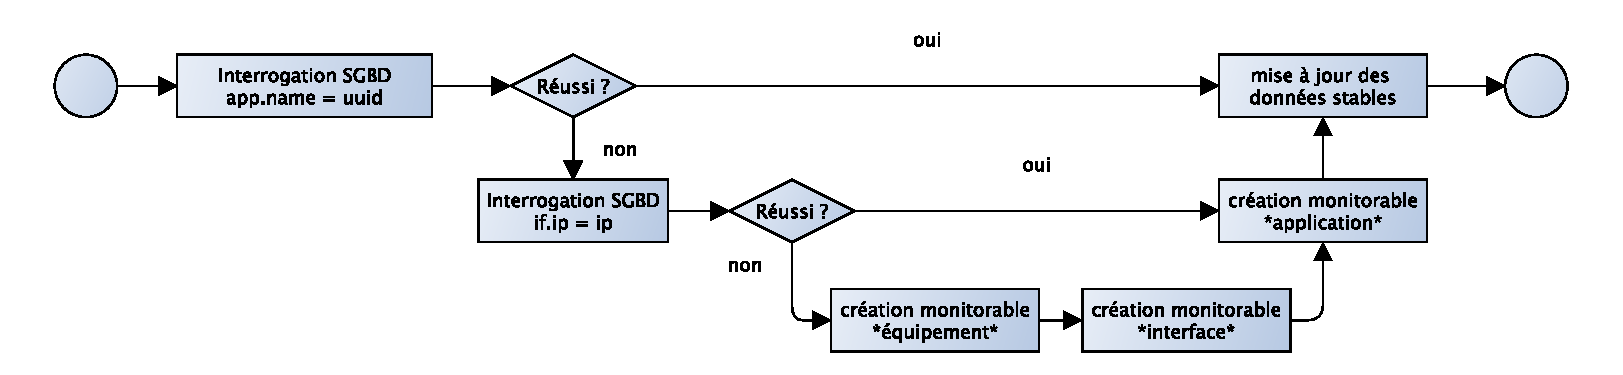
\includegraphics[width=\textwidth]{valid-domvision-statushandler}
	\caption{Description du processus de mise à jour de \textit{StatusSink}}\label{fig:valid:domvision:statushandler}
\end{figure}

Concernant les informations venant d'\textit{UPnP-DM}, nous pouvons les regrouper en un flux $DM$ grâce aux clés de jointures \textit{uuid} et \textit{SystemName}\footnote{Les sources sont synchronisés par le mécanisme d'événement. Sans cette synchronisation un partitionnement \textit{uuid} serait nécessaire.}. Ainsi nous obtenons un flux indiquant que l'interface \textit{SystemName} (avec les propriétés données) est sur l'équipement identifié par le \textit{SerialNumber}. Nous pouvons appliquer la même approche que pour \textit{StatusHandler} en créant un composant puit \textit{DMSink}. La figure~\ref{fig:valid:domvision:cmshandler} résume le processus de ce puit.
$$\begin{array}{c} DM(\textit{uuid},\textit{SerialNumber},\textit{SystemName},\textit{MACAddress},\textit{InterfaceType}, \textit{IPv4Address}, \t)\\
 DM = \IS(\textrm{Serial}[B] \Join \textrm{NetworkInterface}[B] \Join \textrm{IPInterface}[B])\end{array}$$
\begin{figure}[ht]
        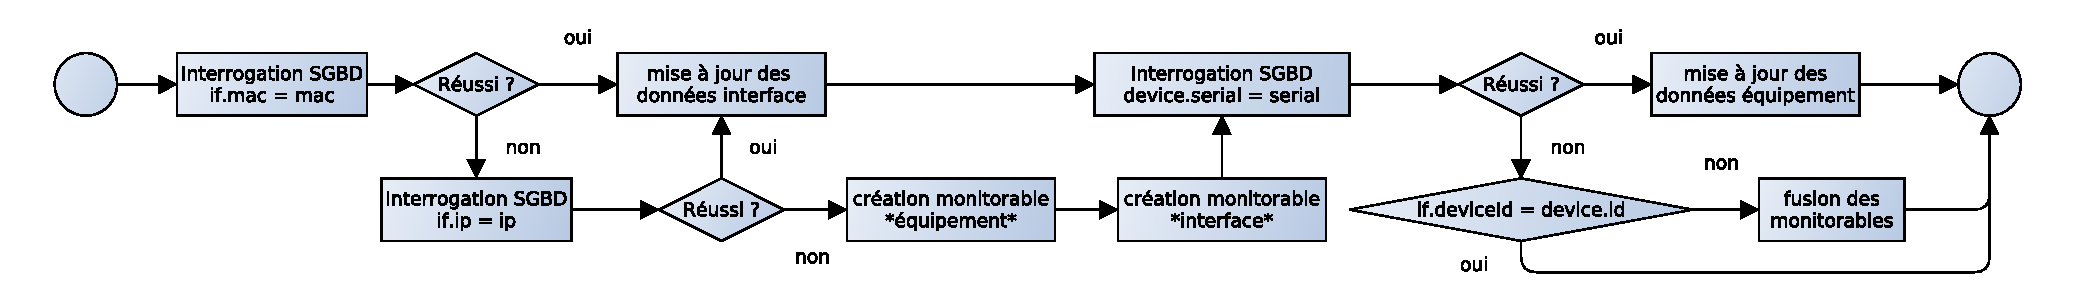
\includegraphics[width=\textwidth]{valid-domvision-cmshandler}
	\caption{Description du processus de mise à jour de \textit{DMSink}}\label{fig:valid:domvision:cmshandler}
\end{figure}

\subsection{Historisation des volatiles}
Nous souhaitons maintenant archiver les données volatiles. Le premier point important à rappeler est que les flux donnés aux composants \textit{VolatilePersistence} doivent être identifiés, i.e. possèdent un attribut \textit{monitorableId}. Ainsi, le flux \textit{OperatingSystem} doit subir une opération pour transformer son \textit{uuid} en \textit{monitorableId} correspondant à l'\textit{équipement} qui le produit. La requête $CPUMem$ fournit le flux avec les attributs $A=$(\textit{CPUUsage}, \textit{MemoryUsage}, \textit{monitorableId},$\t$) répondant à ce problème :
$$CPUMem=\Pi_A \IS(\textit{OperatingSystem}[B]\ssjoin ((\rho_{uuid/monitorableId} \textit{Applications}) \Join \textit{Devices}))$$

Ce flux est donné à une instance de \textit{VolatilePersistence} qui archive dans la table \textit{cpumemhistory} les données volatiles : \textit{cpu} et \textit{memory}. Nous pouvons noter que nous avons fait une jointure avec le catalogue sans difficultés.

Le flux \textit{IPUsage} ne nous donne pas les informations que nous souhaitons. En effet, nous voulons obtenir les données de débit, et le flux fournit un compteur d'octet. Toutefois, nous pouvons transformer une suite de comptage $(c_n,\t_n)$ en série de débits $(d_n,\t_n)$ par l'opération $d_n=\frac{c_n-c_{n-1}}{\t_n-\t_{n-1}}$. L'opérateur $\D_{t>t_0}^{(t,i)^-}$ est capable de revenir un \textit{batch} en arrière, ainsi la requête suivante\footnote{TotalBytesSent et TotalBytesReceived ont été renommés en tbs et tbr pour plus de facilité.} forme le flux voulu :
$$BandwidthUsage = \Pi_{...}\ \IS \left( e_{\frac{tbr-otbr}{\t-o\t}}^{bwr} e_{\frac{tbs-otbs}{\t-o\t}}^{bws}\left(IPUsage[B] \Join \D_{t>t_0}^{(t,i)^-} \rho_{\hspace{-0.33em}\mbox{\tiny $\begin{array}{l} otbs/tbs\\otbr/tbr\\ o\t/\t\end{array}$}}IPUsage[B]\right)\right)$$

Nous avons maintenant le flux possédant les données que nous souhaitons archiver. Comme pour \textit{CPUMem}, nous devons identifier l'entité sur laquelle nous enregistrons cette donnée. Ceci est faisable par une jointure semi-sensible sur la base de données en utilisant le \textit{uuid} de l'agent et le \textit{SystemName} représentant le \textit{nom} de l'interface. Cela produit un flux $Bandwidth$ que nous injectons dans un puit de persistance.

Les autres paramètres volatiles intéressants (changement d'\textit{IP} ou de \textit{status}...) s'enregistrent par le même procédé. D'abord, la requête qui extrait la ou les données que nous souhaitons, puis, identifier l'entité de rattachement.

Nous avons désormais un système d'observation capable d'entretenir sa vision du système et qui archive ses données volatiles. Ces données sont disponibles à travers le SGBD ce qui permet de faire diverses interrogations instantanées avec une capacité d'expression équivalente au \textit{SQL}. Ainsi, nous avons créé un panneau de contrôle indiquant la topologie du réseau ainsi que son histoire et des graphiques de métriques. Une série d'écran est disponible en annexe~\ref{misc:interface}.

\subsection{Formations d'alertes}
Nous montrons maintenant quelques exemples de requêtes continues formant des alertes. La première est une simple sélection sur une valeur limite. Par exemple, nous pouvons supposer que les charges processeurs dépassant le seuil de 90\% sont à notifier à l'utilisateur. Nous pouvons raffiner ce critère par \enquote{\it la moyenne sur 1 minute supérieure à 90\%} afin de lisser les pics de valeurs. Nous pouvons exploiter le flux déjà prêt $CPUMem$ pour effectuer cette requête. Le nouveau flux est ensuite injecté à un composant puit de notification.
$$\IS\ \sigma_{avgcpu>90}(\null_{monitorableId}\G_{avg(CPUUsage)}^{avgcpu} CPUMem[T\ 1min\ 1min])$$

Afin de montrer les capacités d'interrogation de notre système, nous pouvons améliorer cette requête en exprimant le critère \enquote{\it la moyenne sur 1 minute est différente à 10\% près de la moyenne historique}. La valeur historique est obtenue par la relation temporelle produite par $HistAvgCPU=\null_{monitorableId}\G_{avg(cpu)}^{avgcpuhist} cpumemhistory$. Nous obtenons ainsi la requête :
$$\IS\ \sigma_{\abs{avgcpu-avghist}\geq 10}\left(AvgCPU\ssjoin HistAvgCPU\right)$$
